\chapter{ Spread of Zika virus on a small world network }
\Jnote{Title capitalization incosistent with other chapters.}

The deterministic models discussed in the chapters above assume that all individuals have an equally small probability of being infected. In this section we build a model for the propagation of Zika virus based on a small world network.

Traditional models of infectious disease dynamics have a long, successful history of describing and modelling infectious disease spread of many diseases. They are quiet simple and tractable \citep{fu2013propagation}.

They
\Jnote{s/They/There}
are certain specific and common situations when the structure of social connectivity is at least as important as the inactivity of the underlying infectious agents for the study of transmission of infection and control. This is one among the major reasons that has motivated the modelling of infectious diseases on social networks \cite{fu2013propagation}.



\section{ Vector bone disease propagation on a small world network}
We assume that there is a lattice with two layers. One for mosquitoes, another for human beings. A mosquito $M_1$ bites a Zika infected person $h_1$ with probability $\alpha_1$. Then transmits the virus to person $h_2$, with a probability of $\alpha_2$. Thus, person $h_1$ is connected to  person $h_2$ through $M_1$. It can then be said that $h_2$ can be infected by $h_1$ with probability $p_1$, where $p_1 =  \alpha_1 \alpha_2$. Owing to the fact
\Jnote{It is not a fact, but a simplifying assumption we are making.}
that $\alpha_1$ and $\alpha_2$ are  independent. $h_1$ and $h_2$ are said to be near neighbours.

\Jnote{Change order here. First say that we assume mosquitoes are
  stationary and that people have close and remote links. Only then discuss
  probabilities.}

Mosquitoes do not travel long distances, but humans on the other hand travel long distances. If person $h_3$ travels to the place where $h_1$ live or gets close enough that he gets bitten by mosquito $M_1$ and is infected with probability $\alpha_3$. Thus, $\alpha_3$ is the probability that person $h_3$ travels and get bitten by mosquito $M_1$. It can be said that $h_1$ infects $h_3$ with probability $p_2$, because $h_1$ is connected to $h_3$ through $M_1$. Since $\alpha_1$ and  $\alpha_3$ are independent, $p_2 = \alpha_1 \alpha_3$. $h_3$ is said to be a distant neighbour to $h_1$.
\begin{figure}[h!]
\centering
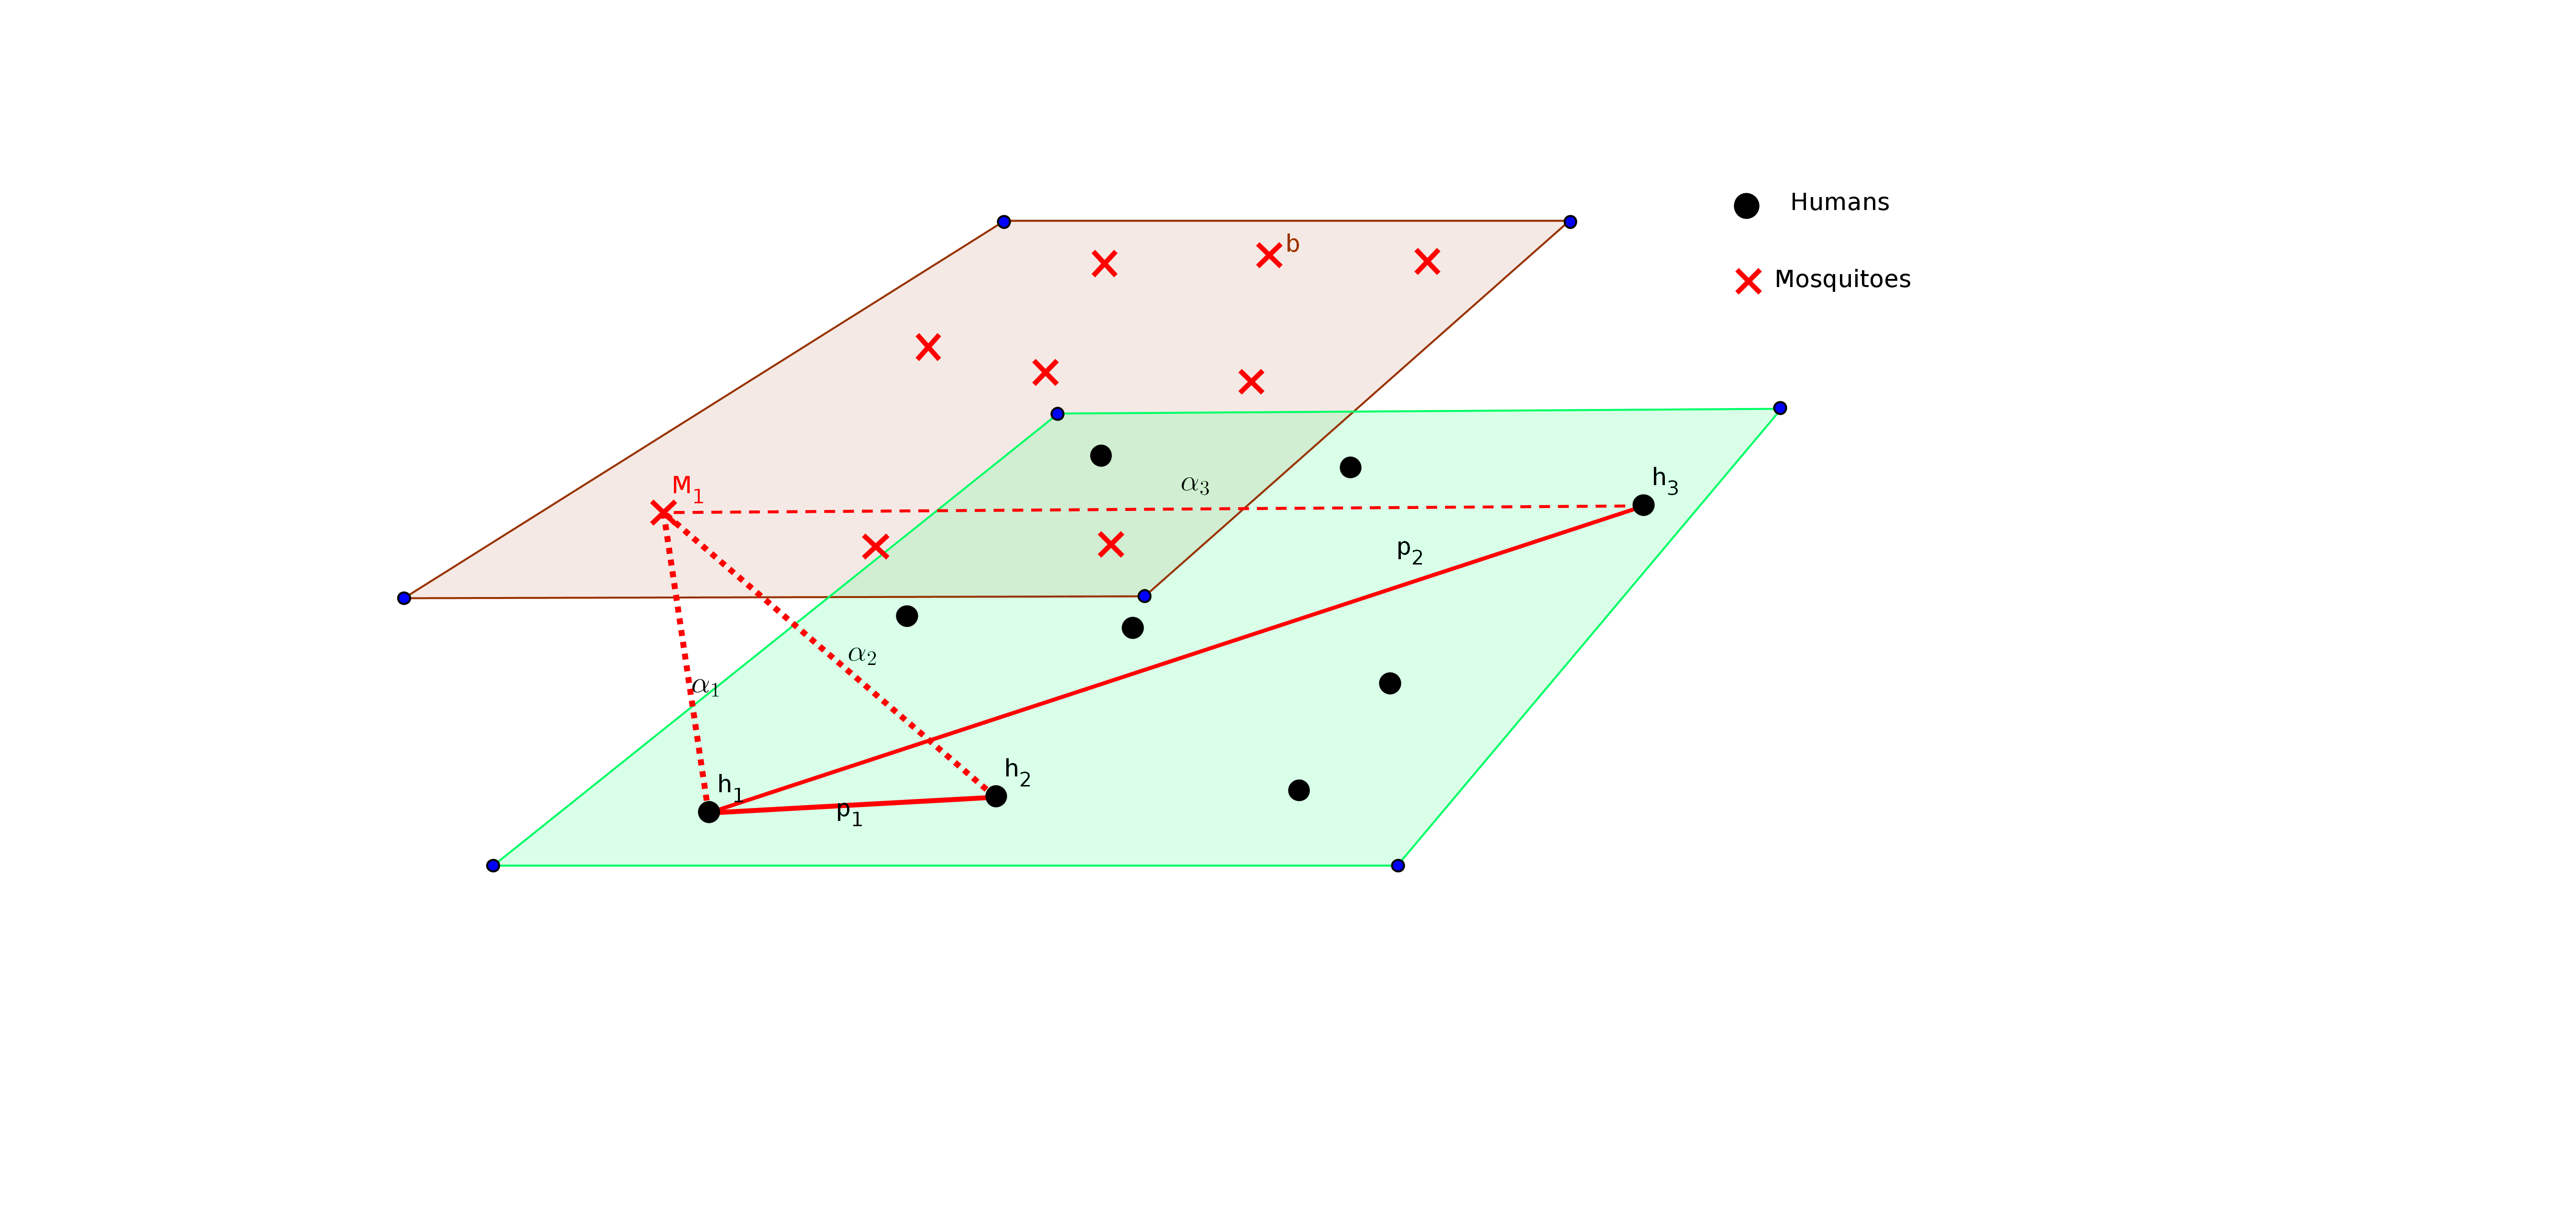
\includegraphics[scale=0.6]{images/human_mosquito.png}
\caption{Disease transmission through a vector} \label{fig5}
\end{figure}
The phenomenon of infecting a distant neighbour can be expressed in 3 cases.
\Jnote{Don't you need 4 cases, also for local-local?}
\begin{itemize}
\item[i.] $h_4$ may travel to a place near enough to get the infection from $h_1$ through $M_1$. In this case $h_3$ is still referred to as a distant neighbour.
\item[ii.] $ h_1$ may travel to a place near enough to infect $h_4$  through another mosquito in that vicinity.In this case $h_3$ is still referred to as a distant neighbour.
\item[iii.] $h_1$  and $h_3$ may both travel to some place at the same time and $h_1$ transmits the infection to $h_3$. In this case $h_3$ is still referred to as a distant neighbour.
  \Jnote{No, we neglect this case.}
\end{itemize}

In all the case we assume $\alpha_3$ is the same. Hence the probability of affecting a remote any distant neighbour neighbour is the same.
\Jnote{Also mention that we assume a single mosquito transmits at most
  one infection.}

The existence of near and distant neighbours in the disease infection dynamics of Zika virus on a lattice with two layers in \ref{fig5} makes it possible to represent the dynamics of disease spread on a small world network in figure \ref{fig 5.2}.Thus, in modelling the spread of Zika virus on a small world network, the dynamics of transmission through mosquitoes are represented by the edges of the graph. An edge is drawn between two vertices, whenever there is a likelihood of transmission from one to another via mosquito bite as can be seen in figure \ref{fig 5.2}.
\begin{figure}[h!]
\begin{minipage}[c]{1\textwidth}
 \centering
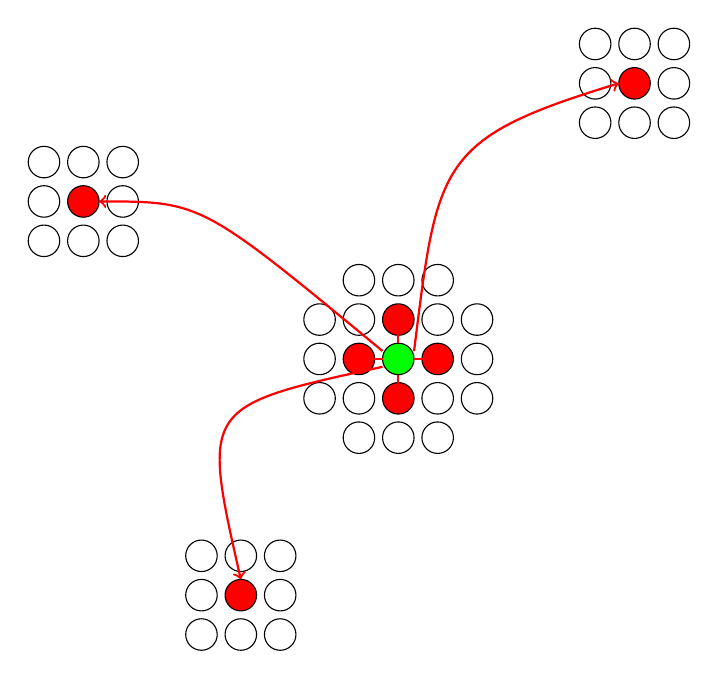
\begin{tikzpicture}
\draw (0,5.5) circle (0.2cm);
\draw (0,5.0) circle (0.2cm);
\draw (0,4.5) circle (0.2cm);
\draw (1,5.5) circle (0.2cm);
\filldraw[fill=red!, draw=black] (0.5,5.0) circle (0.2cm);
\draw (0.5,4.5) circle (0.2cm);
\draw (0.5,5.5) circle (0.2cm);
\draw (1,5.0) circle (0.2cm);
\draw (1,4.5) circle (0.2cm);
\draw (4,2) circle (0.2cm);
\filldraw[fill=red!, draw=black](4,3) circle(0.2 cm);
\draw (4.5,2) circle (0.2cm);
\filldraw[fill =green, draw =black](4.5,3) circle(0.2 cm);
\draw (4,2.5) circle (0.2cm);
\draw(4,3.5) circle(0.2 cm);
\filldraw[fill=red!, draw=black] (4.5,2.5) circle (0.2cm);
\filldraw[fill=red!, draw=black](4.5,3.5) circle(0.2 cm);
\draw (5,2) circle (0.2cm);
\filldraw[fill=red!, draw=black](5,3) circle(0.2 cm);
\draw (5,2.5) circle (0.2cm);
\draw(5,3.5) circle(0.2 cm);
\draw(3.5,2.5) circle (0.2cm);
\draw(3.5,3) circle (0.2cm);
\draw(3.5,3.5) circle(0.2cm);
\draw(4,4) circle(0.2cm);
\draw(5.5,2.5) circle (0.2cm);
\draw (5.5,3) circle (0.2cm);
\draw(5.5,3.5) circle (0.2cm);
\draw(4.5,4) circle(0.2 cm);
\draw(5,4) circle(0.2 cm);

\draw(2,0.5) circle (0.2cm);
\draw (2,0.0) circle (0.2cm);
\draw (2.5,-0.5) circle (0.2cm);
\draw (2.5,0.5) circle (0.2cm);
\filldraw[fill=red!, draw=black](2.5,0) circle (0.2cm);
\draw (2,-0.5) circle (0.2cm);
\draw (3,0.5) circle (0.2cm);
\draw (3,0) circle (0.2cm);
\draw (3,-0.5) circle (0.2cm);


\draw (7,6) circle (0.2cm);
\draw (7,6.5) circle (0.2cm);
\draw (7,7) circle (0.2cm);
\draw (7.5,6) circle (0.2cm);
\filldraw[fill=red!, draw=black](7.5,6.5) circle (0.2cm);
\draw (7.5,7) circle (0.2cm);
\draw (8,6) circle (0.2cm);
\draw (8,6.5) circle (0.2cm);
\draw (8,7) circle (0.2cm);

\draw[red!,thick] (4,3) --(4.3,3);
\draw[red!,thick] (5,3) --(4.7,3);
\draw[red!,thick] (4.5,3.5) --(4.5,3.2);
\draw[red!, thick] (4.5,2.5) --(4.5,2.8);

\draw[draw=red!,
preaction={->,thick,draw =red!}
] (4.7,3.1) ..controls(5,5.5) and (5,5.8) ..(7.3,6.5);
\draw[ draw =red!,thick, ->] (4.3,3.1) .. controls (2,5) and (2,5) ..(0.7,5);

\draw [draw =red , thick, ->] (4.3,2.9).. controls (2,2.4) .. (2.5,0.2);
\end{tikzpicture}
%\caption{Smallworld network structure} \label{fig 5.1}
\end{minipage}
\caption{Smallworld network structure} \label{fig 5.1}
\end{figure}
\section{Small world methodology}

We  can now suppose that the population is arranged in a regular
\Jnote{2-dimensional square}
grid.
Where each vertex can infect its 4 nearest neighbours and a number of distant neighbours. Near neighbours in this case refers to individuals that one spends most of their time could be colleagues at work or school, people in the same house and distant neighbours refers to random individuals that one is likely to transmit the infection to. 
 
 \begin{figure}[h]
 \centering
 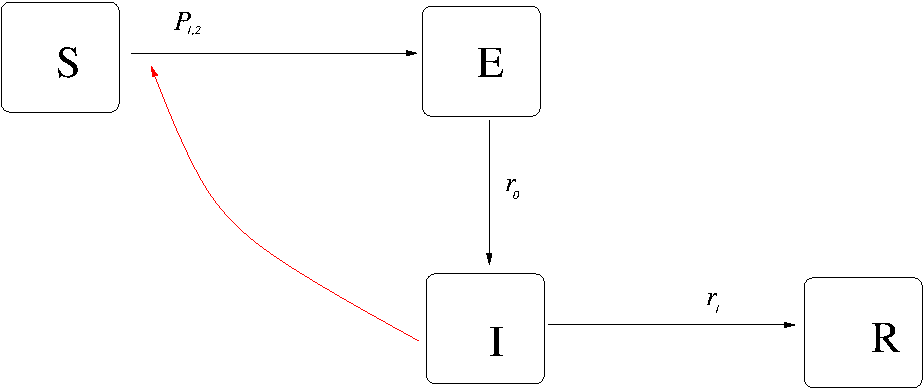
\includegraphics[scale=0.3]{images/swseir.png}
 \caption{State transition diagram} \label{fig 5.2}
\end{figure}
\Jnote{I never liked this picture. If you had time, you could make
  another one that makes clear that all vertices lie on a single grid.}
 
 
 
Figure \ref{fig 5.1} shows the arrangement of nodes in a small world network and figure \ref{fig 5.2} show the transmission state diagram: S to E based on the small world network structure and the infection probabilities $p_ {1,2} $: E to I with probability $r_0$ and I to R with probability $r_1$. in figure \ref{fig 5.1}, the infected green node may infect its four red near neighbours with probability $p_1$ and its three remote neighbours with probability $p_2$. By infection we mean transition from Susceptible to exposed state.

Let $p_1$ be the probability of an infected individual causing their susceptible near neighbours to become infected and $p_2$ the probability of their distant or remote neighbours to become infected. Exposed people become infectious with probability $r_0$ and recover or get removed with probability $r_1$. In addition $n_1$ and $n_2$ is number of close neighbours and near neighbours respectively.
\Jnote{Mention that all probabilities are per day.}
\Jnote{Make clear that $n1=4$ (or less on the borders).}

The number of distant neighbours $n_2$ if fixed and random for each node.
\Jnote{Better say: it is i.i.d.~for each node.}
That is for node I
\Jnote{Don't use I, it means infected. It is typical to use
  $u$ or $v$.}
there are $n_2^ {(I)} $ distant neighbours. $n_2^ {(I)} $ is chosen to follow a discrete exponentially decaying distribution 
\begin{equation} 
  f_c (x) = \dfrac{1}{c} e^{\dfrac{-x}{\mu}} \end{equation}
\Jnote{Write it as
  $\Pr[n_2^{(v)} = k] = c \cdot \exp\left( -\mu x  \right)$.}
with parameter $\mu$ proportional to the expected number of links
\Jnote{I don't think $\mu$ is proportional to that.}
to remote nodes and $c = \frac{1}{1- e^{frac{-1}{\mu}}}$ ensures that $f_c$ is a probability distribution function \citep{fu2013propagation}. The degree distribution in most social networks is exponentially distributed because of the celebrity effect \citep{estrada2015first}. In social networks, there are few people who have a high number of connections and many others with an average number of connections. In modelling infectious diseases these individuals are referred to as supper spreaders.

The transition probability $r_0$, the number of days an individual is in the exposed state is as a result of Bernoulli trials with mean $\frac{1}{r_0}$, follows a geometric distribution $f_X (x) = (1-p) ^ {x-1} p$. Similarly the infectious period follows a geometric distribution with mean $\dfrac{1}{r_o}$ \citep{fu2013propagation}.

\section{Model}
The model has seven parameters, they are $N, p_1, p_2, n_1, n_2, r_0$ and $r_1$. We let $N$ be the population size of a city or country and is arranged in a regular grid of side length $l $ such that $l^2 = N$. The rest of the parameters have been described above.
\Jnote{I wouldn't say $n_1$ is a parameter, it is always $4$ for us.}

A thorough review of literature in \cite{lessler2016times} indicates that $95 \%$ of patients
\Jnote{What do you mean by $95\%$ of patients? I think you are confused here.}
  begin to exhibit symptoms of Zika infection after $11.2$ days of infection with a $95 \%$ confidence interval of $7.6 -18$. Further the center for disease control and prevention (CDC) indicate that the incubation period for the Zika virus ranges from 3 days to 14 days from infection \citep{krow2017estimated}. Therefore we estimate $r_o$ with $\frac{1}{11.2}$\
  \Jnote{These are the values before you exhibit symptoms. Are they the same
    for becoming infective?}
  \Jnote{Consider adding some days to allow time for a mosquito to transmit
    the virus.}

  $95\%$ of the cases will still have detectable virus infectiousness 18.9 days after infection with a confidence interval of 13.6 -79.4 \citep{lessler2016times}.The infectiousness in Zika infection ends 1.5 - 2 days before the virus becomes undetectable \citep{funk2016comparative}. Thus the chosen value of the infectious period is $18.9 - 1.5 = 17.4$ days. Therefore $r_1$ is estimated to be $\frac{1}{17.4}$.
  \Jnote{If you have time, please try different $r1$ since the confidence
    interval is large.}

Hence we have $n_1$, $\mu$, $p_1$ and $p_2$ free parameters. Without control. Since the average number of secondary infections resulting from a primary  Zika  virus infectious is between 3 and 6, therefore we choose 4.5 as the $R_0$. Since the number of remote neighbours is random and fixed for each, we estimate $E (n^ {(I)} _2) = \mu$.

\Jnote{Please explain equations below.}
\begin{align}
n_1 p_1 + \mu p_2 \approx \dfrac{R_0}{r_1} 
\\ n_1 p_1 + \mu p_2 \approx 0.2586 \label{eqn 5.32}
\end{align}
thus, 
$p_1 \approx   0.0645- 0.25 \mu p_2$

We can summarize the parameters of the models as;
\begin{align}
n_1 &= 4 \\
\mu &= 8 \\
r_0 &= \dfrac{1}{11.2} \approx 0.089 \\
r_1 &= \dfrac{1}{17.4} \approx 0.057 \\
p_1 &= 0.0645 - 2 p_2 \label{eqn 5.1.7}
\end{align}
Now we have one free parameter. We can now estimate the number of new infections by;
\begin{align}
E(- \bigtriangleup S) = (n_1 k p_1 + \mu p_2 - r_1) I \label{5.18}
\end{align}
Where k is the average number of near neighbours' links that support possible infection and near neighbours are arranged in clusters, therefore $0.5 k 1$.  In our computation, we will take $k = 0.5$. From equation \ref{5.18} we can estimate the number of new infections as;
\begin{align}
E(- \bigtriangleup S) = (2 p_1 + 8 p_2 - 0.057) I  \label{5.1.9}
\end{align}
 
From equation \ref{eqn 5.32}, it can be shown that $p_1$ and $p_2$ have natural bounds. That is taking $p_2 = 0$, implies that $p_1 \leq 0.1293$ for $k =0. 5$. For $p_1 = 0$, we get $p_2 \leq 0.3232$.
\section{Simulation}
To investigate how disease propagation varies depending on $p_1, p_2, $ and $r_1$ we ran a couple of simulation on a small work network.
 
